
\documentclass[xcolor=dvipsnames]{beamer}

% Load the custom theme
\usepackage{iiththeme}
\usepackage{calligra}
\usepackage{amsmath}
\usepackage{graphicx}
\usepackage{booktabs}


% Presentation information
\title[Paper Presentation]{LLM-Text Watermarking based on Lagrange Interpolation}

\author[Manoj Kumar]{
	\vspace{-0.2cm}
	\textbf{Manoj Kumar V K} \\
	\vspace{0.2cm}
	{\small Under the Guidance of \\ 
	\textbf{Dr. Shibam Ghosh}}
}

\institute[IIT Hyderabad]{
	Department of Computer Science\\
	Indian Insitute of Technogology Hyderabad
}

\date{\today}

\begin{document}
	
	% Title slide: title, logo, author, institute, date
	\begin{frame}
		\titlepage
	\end{frame}
	
	% Table of contents
	\begin{frame}
		\tableofcontents
	\end{frame}
	
	% Section 1
	\section{Introduction}
	
	\begin{frame}{Introduction}
		\begin{itemize}
			\item LLM-generated text can be modified, paraphrased,
			truncated, or partially deleted.
			
			\item Such modifications can disrupt watermark detection
			and authorship attribution.
			
			\item Watermarking embeds identifiable information into
			generated text without requiring a visible signature.
			
			\item \textbf{Problem:} Recover the embedded author identity
			even when only part of the original text survives.
		\end{itemize}
	\end{frame}
	
	\begin{frame}{Research Gaps}
		\begin{itemize}
			\item Recovering a specific author's identity is more
			demanding than simply detecting a watermark.
			
			\item Text modifications can corrupt or remove embedded
			watermark information.
			
			\item The verifier must distinguish genuine watermark
			points from corrupted or spurious points.
			
			\item Reliable recovery requires a balance between
			robustness, computational efficiency, and security.
		\end{itemize}
	\end{frame}
	
	\begin{frame}{Contributions}
		\begin{itemize}
			\item A Lagrange interpolation-based scheme that encodes
			an author's identity in a straight line over a finite field.
			
			\item A Maximum Collinear Points (MCP) approach to recover
			the watermark from potentially corrupted points.
			
			\item A security analysis of accidental collinearities
			and algebraic attacks.
			
			\item Extraction variants and extensions to multiple
			secrets and higher-degree polynomials.
			
			\item Experimental evaluation of random point sets over
			finite fields of different sizes.
		\end{itemize}
	\end{frame}
	
	\section{Methodology}
	
	\begin{frame}{Proposed Watermarking Scheme}
		\begin{enumerate}
			\item Encode the secret identity as coefficients of
			a polynomial over $GF(2^n)$.
			
			\item Generate pseudorandom coordinates $x_i$ using
			a secret-seeded generator.
			
			\item Compute watermark points $(x_i,f(x_i))$.
			
			\item Embed the bits of these points into the generated
			text by biasing token-selection logits.
			
			\item Recover candidate points from the text and use
			MCP to identify the dominant line.
			
			\item Reconstruct the secret identity from the line's
			coefficients.
		\end{enumerate}
	\end{frame}
	
	\begin{frame}{Watermark Representation}
		\begin{itemize}
			\item All polynomial operations are performed over
			the finite field $GF(2^n)$.
			
			\item The secret identity is represented by the
			coefficients of a linear polynomial:
			\[
			f(x)=a_0+a_1x
			\]
			\[
			K=(a_0\parallel a_1)
			\]
			
			\item Generate pseudorandom coordinates using an
			LFSR with secret seed $sk$:
			\[
			x_i=\operatorname{LFSR}(t_i,sk)
			\]
			
			\item Compute the corresponding watermark points:
			\[
			P_i=(x_i,y_i),\qquad y_i=f(x_i)
			\]
			
			\item Each point encodes $2n$ bits; $N$ points require
			\[
			T=2nN \text{ bits}.
			\]
		\end{itemize}
	\end{frame}
	
	\begin{frame}{Embedding Watermark Bits into Text}
		\begin{itemize}
			\item Partition the vocabulary into two subsets:
			\[
			V=V_0\cup V_1,\qquad V_0\cap V_1=\varnothing
			\]
			
			\item Tokens in $V_0$ represent bit $0$, while tokens
			in $V_1$ represent bit $1$.
			
			\item Modify token-selection logits to favor tokens
			corresponding to the desired watermark bit.
			
			\item The embedding procedure encodes both $x_i$ and
			$y_i=f(x_i)$ into successive token blocks.
			
			\item The text remains naturally generated, while
			token choices carry the watermark information.
		\end{itemize}
	\end{frame}
	
	\begin{frame}%{Watermark Embedding (Algorithm 1)}
		\centering
		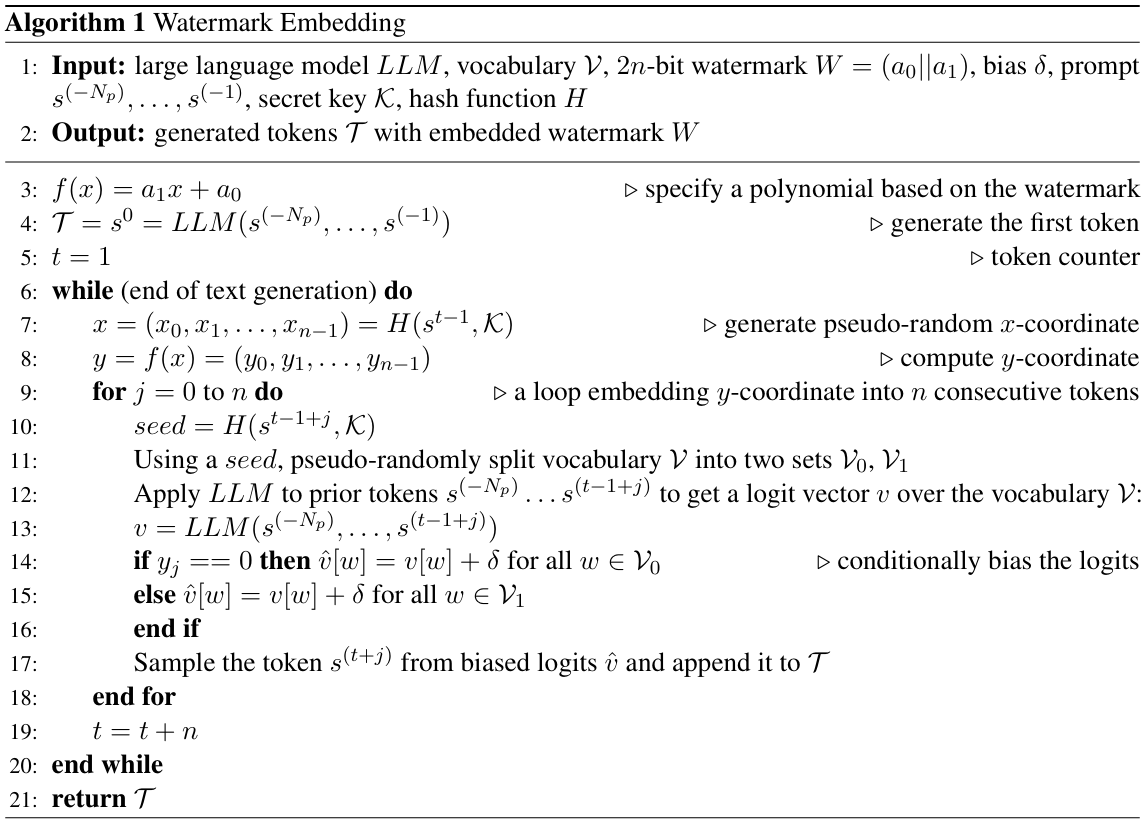
\includegraphics[
		width=\textwidth,
		height=0.95\textheight,
		keepaspectratio
		]{images/algorithm1.png}
	\end{frame}
	

	\begin{frame}%{Watermark Extraction (Algorithm 2)}
		\centering
		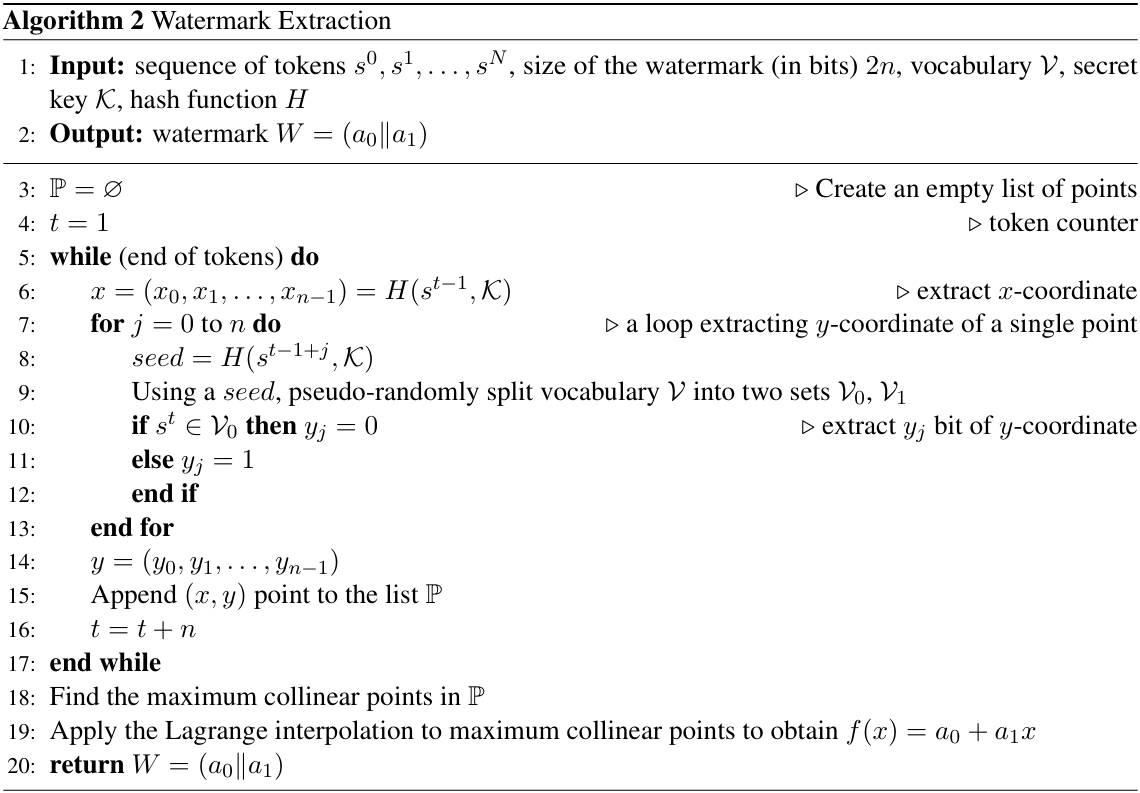
\includegraphics[
		width=\textwidth,
		height=0.95\textheight,
		keepaspectratio
		]{images/algorithm2.png}
	\end{frame}
	
	\begin{frame}{Maximum Collinear Points (MCP)}
		\begin{itemize}
			\item Text modification may produce both genuine and
			corrupted watermark points.
			
			\item Genuine points lie on the original line:
			\[
			f(x)=a_0+a_1x
			\]
			
			\item The MCP problem finds the largest subset of
			points lying on a common straight line.
			
			\item The line with the largest number of recovered
			points is considered the watermark candidate.
			
		\end{itemize}
	\end{frame}
	
	\section{Extraction Variants}
	
	\begin{frame}{Simplified Watermark Extraction}
		\begin{itemize}
			\item \textbf{Standard extraction}
			\begin{itemize}
				\item Use the secret-keyed LFSR to identify valid
				$x_i$ coordinates.
				\item Extract the corresponding $f(x_i)$ values.
				\item Apply MCP to the recovered points.
			\end{itemize}
			
			\item \textbf{Simplified extraction}
			\begin{itemize}
				\item Slide a $2n$-bit window across the extracted
				watermark bit sequence.
				\item Interpret each window as a candidate point.
				\item Apply MCP directly to all candidate points.
			\end{itemize}
			
			\item This avoids filtering candidates using valid
			LFSR-generated coordinates but introduces more
			spurious points.
		\end{itemize}
	\end{frame}
	
	\begin{frame}{Double-Resolution Watermarking}
		\begin{itemize}
			\item Consecutive points can be constructed using
			repeated applications of the linear function:
		\end{itemize}
		
		\[
		f(x)=a_0+a_1x
		\]
		
		\[
		(x,f(x)),\;
		(f(x),f^2(x)),\;\ldots,\;
		(f^{N-1}(x),f^N(x))
		\]
		
		\begin{itemize}
			\item Consecutive points share coordinates, reducing
			the number of candidate points produced by sliding
			windows.
			
			\item Candidate count decreases from
			$2n(N-1)+1$ to $n(N-1)+1$.
			
			\item Short cycles may require a new initial value;
			the security implications must also be considered.
		\end{itemize}
	\end{frame}
	
	\section{Security Analysis}
	
	\begin{frame}{Security Analysis: Watermark Recovery}
		\begin{itemize}
			\item Let $N=F+R$, where:
			\begin{itemize}
				\item $F$: genuine points lying on the secret line.
				\item $R$: random or corrupted points.
			\end{itemize}
			
			\item The analysis models corrupted points as randomly
			distributed over $GF(2^n)\times GF(2^n)$.
			
			\item Recovery is reliable when the genuine line contains
			more points than any competing line formed by corrupted
			points.
			
			\item Larger finite fields reduce the probability of
			accidental collinearities under this model.
		\end{itemize}
		
		\vspace{0.15cm}
		\[
		f(x)=a_0+a_1x,\qquad K=(a_0\parallel a_1)
		\]
	\end{frame}
	
	\begin{frame}{Algebraic Attack and Countermeasures}
		\begin{itemize}
			\item \textbf{Vulnerability:}
			An LFSR and fixed token partitions can expose linear
			relationships in the watermark construction.
			
			\item \textbf{Potential attack:}
			An adversary may construct linear equations from
			observed token occurrences to infer the LFSR seed
			and watermark bits.
			
			\item \textbf{Countermeasures}
			\begin{itemize}
				\item Replace the LFSR with a nonlinear feedback
				shift register (NFSR).
				\item Use dynamic token partitions rather than
				fixed $V_0$ and $V_1$.
				\item Derive partitions using cryptographic hashes
				and the secret key.
			\end{itemize}
			
			\item Stronger security may introduce additional
			computational overhead.
		\end{itemize}
	\end{frame}
	
	\section{Evaluation}
	
	\begin{frame}{Experimental Setup}
		\begin{itemize}
			\item \textbf{Objective:} Evaluate the maximum number
			of accidental collinear points in random point sets.
			
			\item \textbf{Method:} Generate random points over
			finite fields of different sizes.
			
			\item \textbf{Fields:}
			\[
			GF(2^6),\ GF(2^8),\ GF(2^{12}),\
			GF(2^{16}),\ GF(2^{32})
			\]
			
			\item \textbf{Evaluation:} Measure the maximum number
			of collinear points for varying numbers of random points.
			
			\item \textbf{Goal:} Study how field size affects the
			likelihood of accidental watermark-like structures.
		\end{itemize}
	\end{frame}
	
	\begin{frame}{Experimental Results}
		\centering
		\scriptsize
		
		\begin{tabular}{r|ccccc}
			\toprule
			\textbf{Random Points} &
			$GF(2^6)$ & $GF(2^8)$ & $GF(2^{12})$ &
			$GF(2^{16})$ & $GF(2^{32})$ \\
			\midrule
			8    & 3  & 2  & 2 & 2 & 2 \\
			16   & 3  & 3  & 2 & 2 & 2 \\
			32   & 5  & 3  & 2 & 2 & 2 \\
			64   & 6  & 4  & 3 & 2 & 2 \\
			128  & 6  & 5  & 3 & 2 & 2 \\
			256  & 10 & 5  & 3 & 2 & 2 \\
			512  & 14 & 8  & 3 & 2 & 2 \\
			1024 & 20 & 11 & 4 & 2 & 2 \\
			\bottomrule
		\end{tabular}
		
		\vspace{0.3cm}
		\begin{itemize}
			\item Small fields exhibit more accidental collinearities.
			\item For $GF(2^{16})$ and $GF(2^{32})$, the observed
			maximum remains two in these experiments.
			\item Larger fields make accidental watermark-like
			structures less likely in the tested random sets.
		\end{itemize}
	\end{frame}
	
	\section{Extensions}
	
	\begin{frame}{Multiple Secrets and Higher-Degree Polynomials}
		\begin{itemize}
			\item \textbf{Multiple lines as secrets}
			\begin{itemize}
				\item Embed multiple lines, each encoding a distinct
				secret.
				\item Recover the top $t$ lines using MCP.
				\item Establish a deterministic ordering before
				concatenating the secrets.
			\end{itemize}
			
			\item \textbf{Higher-degree polynomials}
			\[
			f(x)=a_0+a_1x+\cdots+a_dx^d
			\]
			\begin{itemize}
				\item Encode the secret in the polynomial coefficients.
				\item Reconstruct the polynomial using Lagrange
				interpolation.
				\item Identify genuine points using Maximum
				Co-Polynomial Points (MCPP).
			\end{itemize}
		\end{itemize}
	\end{frame}
	
	\section{Conclusion}
	\begin{frame}{Conclusion and Future Work}
		\begin{itemize}
			\item \textbf{Conclusion:}
			\begin{itemize}
				\item Proposes Lagrange interpolation-based watermarking to encode author identity in LLM-generated text.
				\item Uses MCP to recover the watermark from potentially modified text.
				\item Improves security using cryptographically stronger pseudorandom generation and dynamic token partitions.
				\item Supports extensions to multiple secrets and higher-degree polynomials.
			\end{itemize}
			\item \textbf{Future work:}
			\begin{itemize}
				\item Improve resilience against adversarial text modifications.
				\item Optimize recovery of multiple secrets.
				\item Explore hybrid schemes combining lines and higher-degree polynomials.
			\end{itemize}
		\end{itemize}
	\end{frame}
	
	\section{References}
	\begin{frame}{References}
		\tiny\bibliographystyle{alpha}
		\bibliography{references}
		\nocite{*} 
	\end{frame}
	
	\begin{frame}
		\begin{center}
			{\Huge\calligra Thank You}
		\end{center}
	\end{frame}
	
\end{document}
